\documentclass[11pt,a4paper]{article}
\usepackage[margin=2.5cm]{geometry}
\usepackage{amsmath,amssymb,booktabs,xcolor,enumitem,graphicx}
\usepackage[normalem]{ulem}
\usepackage[hidelinks]{hyperref}
\setlength{\parskip}{0.6em}\setlength{\parindent}{0pt}
\definecolor{newc}{HTML}{1f6f43}
\newcommand{\new}[1]{\textcolor{newc}{#1}}
\newcommand{\old}[1]{\textcolor{gray}{\sout{#1}}}
\newcommand{\mockup}[1]{\textit{#1}}
\title{Proposed change [A93], the loop figure and the text around it}
\date{13 November 2026, version 3 (blocking cost and crowding feature, Part~1 and 2.3 to 2.5)}
\begin{document}
\maketitle

\section*{How to read this}
Part~1 says why the figure changes. Part~2 shows the section ``How the two
layers close the loop'' as it would read. \new{Green} is new text, \old{struck}
text goes, black text stays. Part~3 has the questions. Only the RQ number is
changed in the thesis so far, and the RQ numbers.

\section*{Part 1. Why the figure changes}

\subsection*{What the reader already has}
\begin{itemize}[leftmargin=1.2em]
\item \textbf{The loop in words.} The Introduction already explains both
  directions, and that demand storage runs one way while closing the loop runs
  both ways. This section is the second time the reader meets the loop.
\item \textbf{The two clocks.} The environment step figure of the
  Implementation chapter (\texttt{methodloop.pdf}) shows every step against the
  storage epoch.
\item \textbf{The tea example} of Figure \texttt{storageexample}, with two
  aisles, a workstation and new tea placed by demand storage.
\item \textbf{The agents' own crowding feature} $\delta$ of Figure
  \texttt{congestion}. It is easy to confuse with what storage reads.
\end{itemize}

\subsection*{What the reader is missing}
The storage section ends about 500 lines earlier, so the reader has forgotten
its details. ``Standing still at a shelf'' has only been said in words. It is
the one new idea of the section, and no figure in the thesis shows it.

\subsection*{What the old figure did}
It drew boxes and arrows with symbols ($x^{\mathrm{in}}_t$, $\tau_j$,
$\hat\mu_t$). The idea itself is already in the Introduction and in the
section's own words. The figure repeated the abstract part and left out the
concrete part. It also did not show demand storage, so the caption had to.

\subsection*{The new figure}
One figure, two panels. It carries the tea example of Figure
\texttt{storageexample} one storage period further, drawn in the same way.
Shelves are slot boxes hanging off the aisle, and agents stand only on
vertices, as in Figure \texttt{storageupdate}. (a)~Demand storage sends every
tea pick to shelf A, the nearest. Agent $a_1$ picks there while $a_2$ and $a_3$
wait their turn on the aisle. (b)~Congestion-aware storage reads that. The next
line takes C, 6 edges from the workstation against 4 for A, because
$6 + 1 < 4 + 5$. At the next update the new tea goes to the empty shelf of the
quiet aisle. The numbers are those of the pickup
example in ``Orders and tasks''. The corner of Figure \texttt{taskroute} was
tried first, but every trip to $W_1$ passes the same two vertices there, so a
second tea shelf could not be quiet.

\begin{center}
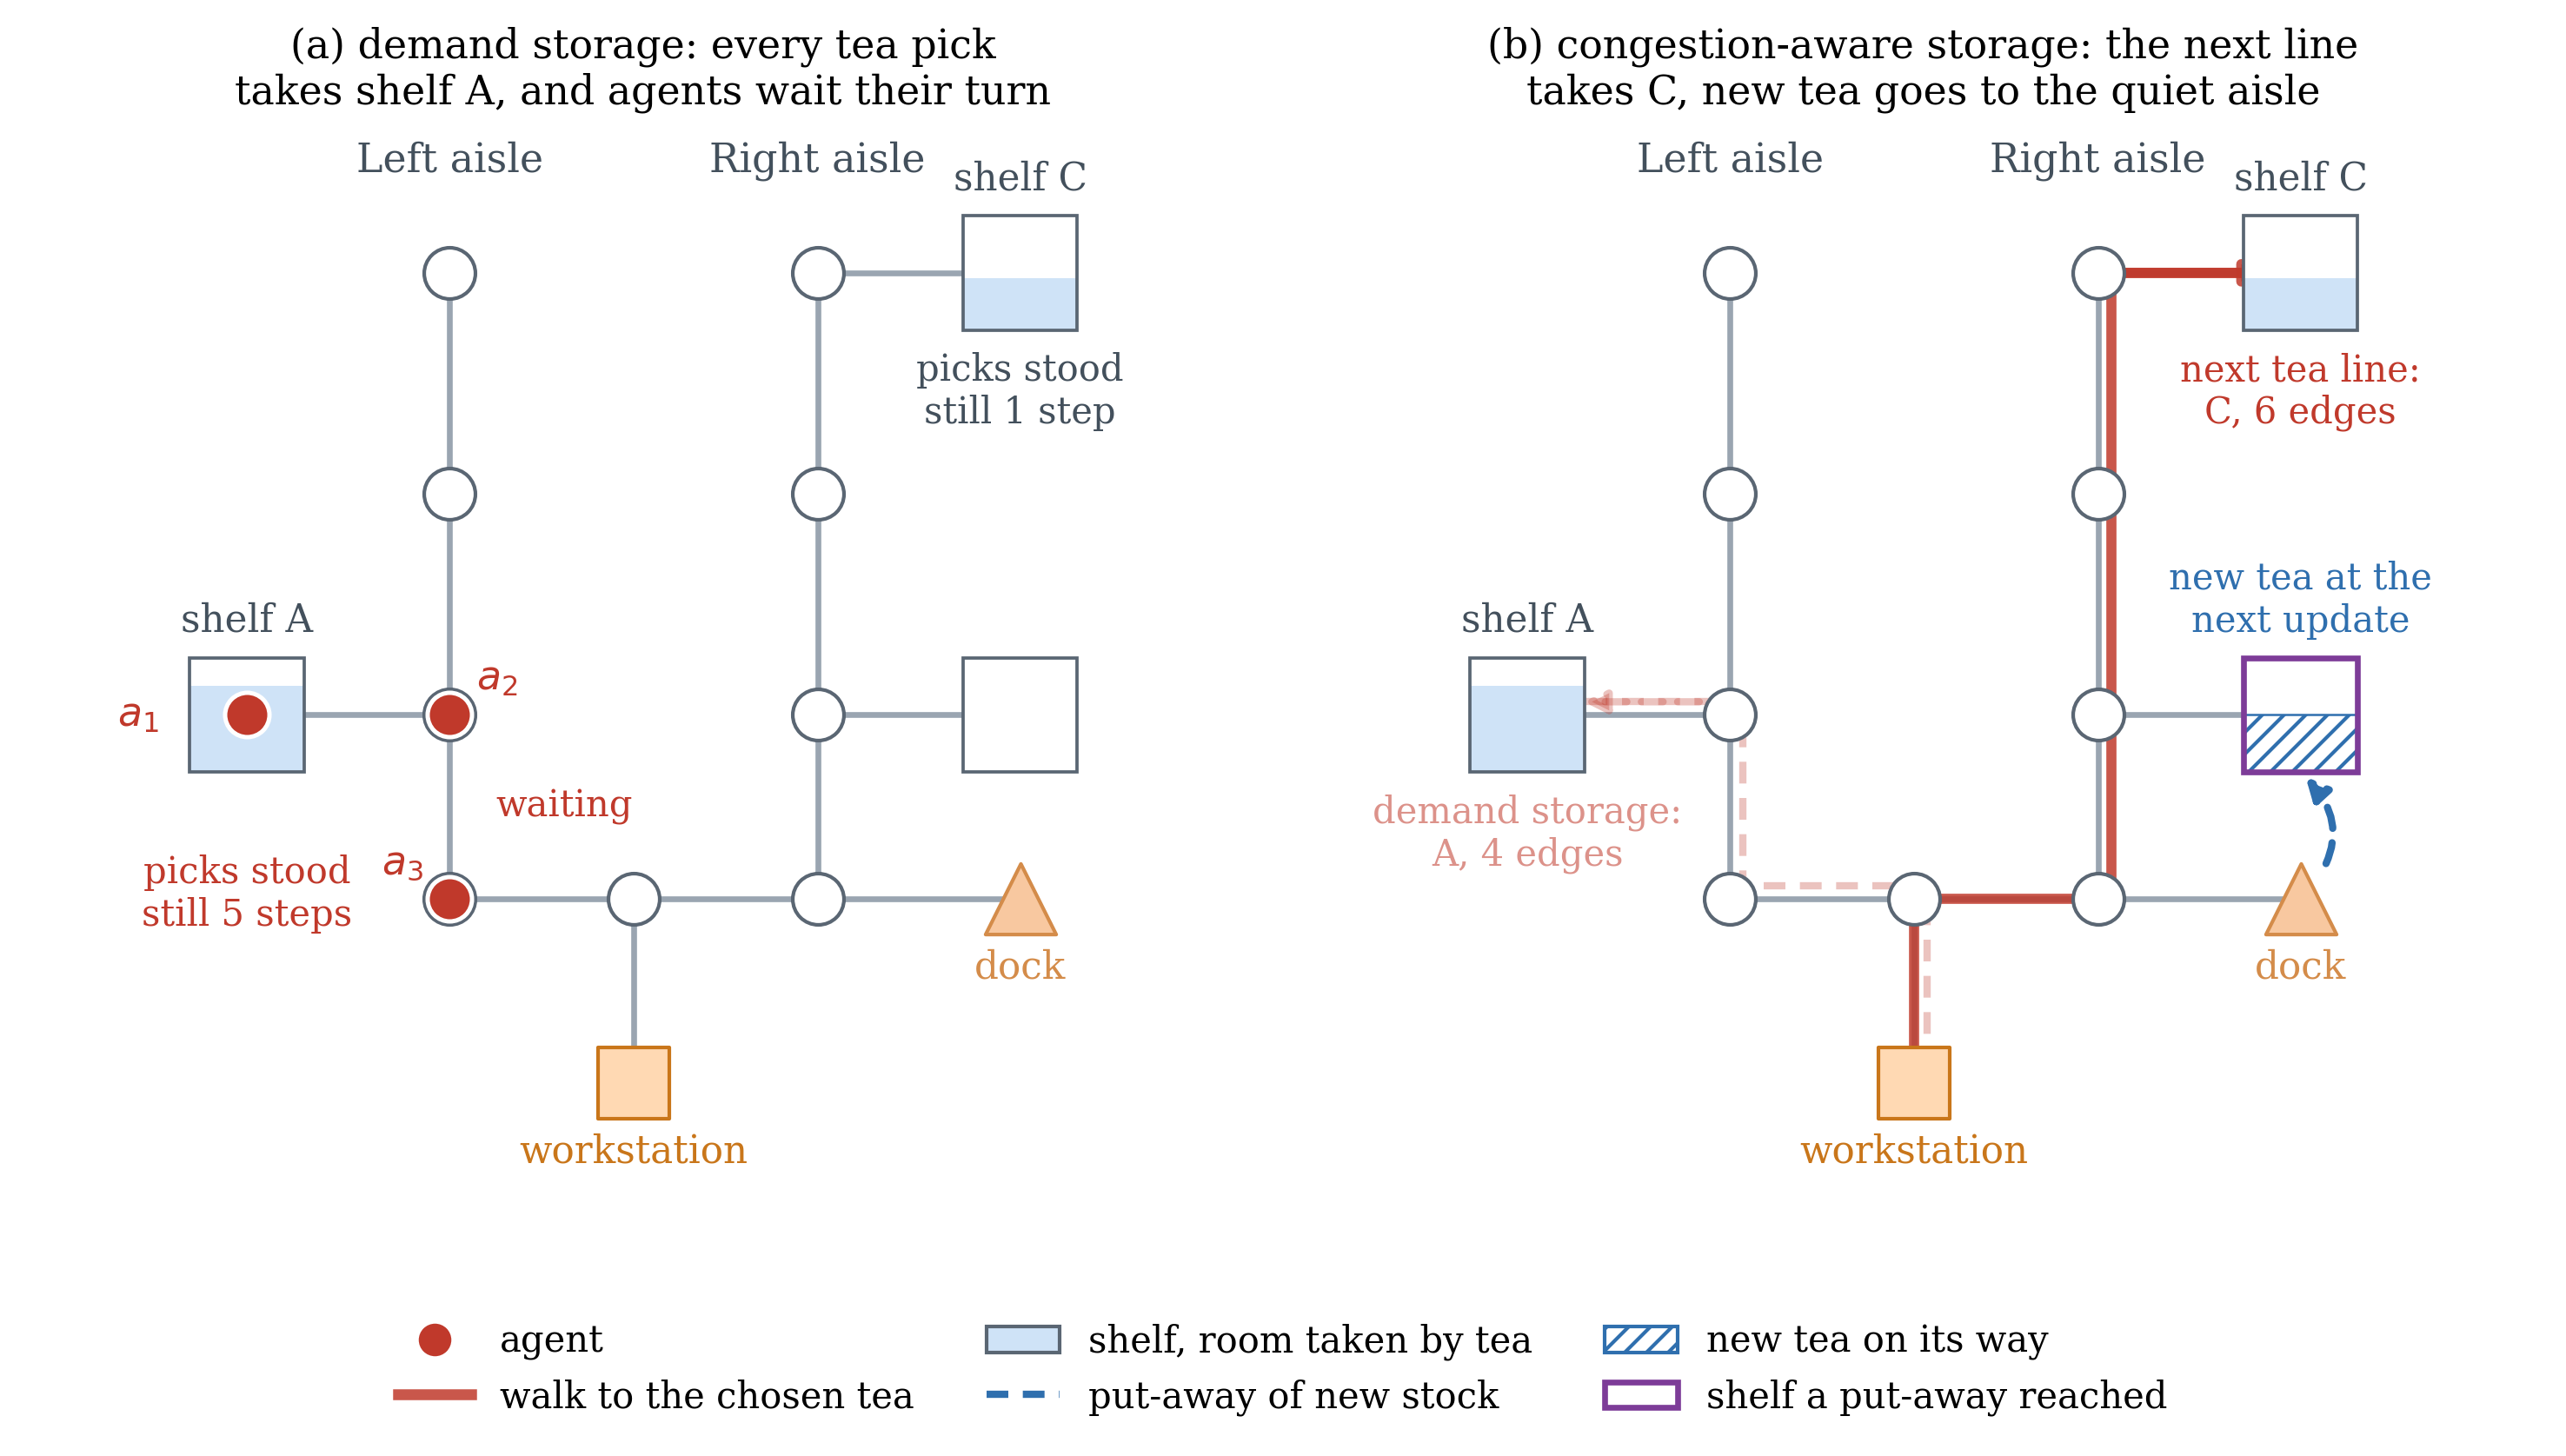
\includegraphics[width=\linewidth]{../../../scripts/Images/shelf_loop.png}
\end{center}

\subsection*{One name per idea}
``Crowding'' meant two things. The share of an agent's view taken by other
agents, $\delta_i(t)$, and the cost $K$ of the storage rule. Since [A93], $K$ is
built from the time picks stood still, so it charges blocking, not crowding. The
thesis already says crowding without blocking costs nothing. $K$ also had a
second name, ``congestion term'', and $\delta_i(t)$ had two, ``congestion
feature'' and ``crowding number''. Now each idea has one name.

\begin{center}
\begin{tabular}{ll}
\toprule
idea & name \\
\midrule
$\delta_i(t)$, what an agent sees around it & crowding feature \\
$\hat\omega_t(v)$, steps picks stood still at a shelf & standing still \\
$K$, built from $\hat\omega_t$ & blocking cost \\
the rule and its weight $\beta$ & congestion-aware storage, congestion weight \\
\bottomrule
\end{tabular}
\end{center}
``Blocking cost'' matches the blocked part of eq.~split, which $\hat\omega_t$
averages, and the blocked time RQ2 asks about. ``Waiting cost'' was not used,
because waiting already names a task waiting for an agent. The labels
\texttt{eq:congestion} and \texttt{fig:congestion} stay, since the reader does
not see them.

\subsection*{Why storage does not read the crowding feature}
A crowd that keeps moving costs no time, and a busy aisle that flows is often the
best place for popular stock. Standing still counts only time that is lost. It
is in steps, the unit of a trip, so $\beta = 1$ has a plain meaning, while
$\delta$ is a share from 0 to 1 and would need a tuned weight. It is booked on
the shelf a pick came from, so it also catches a queue at the workstation. And it
is what RQ2 measures. A storage rule on $\delta$ itself was never run. The
nearest test, passes per edge, did no better than demand storage with Token
Passing on 10 seeds.

\section*{Part 2. The text}

\subsection*{Problem Formulation, ``How the two layers close the loop''}

The two layers of the warehouse run at different speeds. Routing acts on
every timestep. Only every $\Delta$ timesteps, at the storage epochs, does
new stock arrive and the storage rule place it, through eq.~storageupdate.

The two layers influence each other in both directions, and that is what
closes the loop. Forward, storage shapes routing. Placing stock changes
which vertices can be pickups under the stock condition, and so changes where
the agents have to go.

Backward, routing shapes storage. \new{When many picks go to one shelf, the
agents wait their turn there.} How long \old{agents} \new{picks} stand still
is measured at each shelf in $\hat\omega_t$. At the next storage update the
rule uses it to decide where new stock goes, and every new order line uses it
to choose the shelf it picks from. \new{This is not the crowding an agent sees
around itself, the crowding feature of Figure \texttt{congestion}, which only the
controller reads. Storage reads standing still instead, because a crowd that
keeps moving costs no time.
Figure~\texttt{loop} carries the tea example of Figure \texttt{storageexample}
one storage period further, with the numbers of the pickup example in
Section~\texttt{pf:tasks}.}

\mockup{Figure: shelf\_loop.png, at 0.9 of the line width, label fig:loop kept.
Caption:} \new{The tea example of Figure \texttt{storageexample} a period later.
Picks wait at A, so the next line and the new tea go to the quiet aisle.}
\old{The two-timescale loop under fixed (a) and congestion-aware storage (b).
Demand storage reads only $\hat\rho_t$, so standing still never reaches it.}

With fixed storage only the forward path exists. \new{Demand storage places
stock by the orders, and the orders come from customers, not from how the
agents move. So with demand storage the coupling still runs one way, as a gain
that depends on the controller.} The backward path is what congestion-aware
storage adds, because only that rule reads the time agents stand still.
\old{Demand storage follows the orders alone. With demand storage the coupling
therefore shows only one way, as a gain that depends on the controller.} The
loop is closed only in \old{RQ3} \new{RQ2}, which tests it at the main load and
at a higher load where the aisles are crowded. \old{Figure~
\texttt{loop}
  shows this. The fixed-storage baseline comes first, and the congestion-aware
model is the same diagram with the backward path added.}

Separating the two clocks has one consequence that constrains the study.
\mockup{The paragraph on $\Delta$ stays as it is.}

\subsection*{Implementation, ``Where arriving stock goes''}
\ldots{} The gap between the last two shows what reading the time agents stand
still adds to demand alone, which is the storage half of \old{RQ3} \new{RQ2}.

\subsection*{2.3 Problem Formulation, ``What the rule decides''}
The \old{crowding} \new{blocking} cost is this thesis's own, because the classic
problem has no traffic. It adds up, over the same units, how often their SKU is
ordered times how long picks stand still at their shelf. \ldots

\subsection*{2.4 The other places of $K$}
\textbf{Background, ``Congestion and emergence''.} There are two ways to respond
that matter here. The first gives every controller an explicit crowding signal
instead of hoping the fleet corrects itself. The \old{congestion}
\new{crowding} feature does this for routing, and the \old{congestion term}
\new{blocking cost} $K$ \new{does it for storage, through the time picks stood
still. Routing can then react to crowding before it costs time, and storage to
the time it has already cost.} \old{does it for storage. Both layers can then
react to crowding before it costs time.}

\textbf{Problem Formulation, ``Crowding''.} \ldots{} The storage rule guards
against it through the \old{congestion term} \new{blocking cost} $K$ \ldots

\textbf{Notation table.} $D, K$: Its two terms, the slotting cost and the
\old{crowding} \new{blocking} cost. $\beta$: How much the \old{crowding}
\new{blocking} cost $K$, steps standing still, counts against the slotting
cost $D$.

\subsection*{2.5 The crowding feature $\delta_i(t)$}
The same change, \old{congestion feature} or \old{crowding number} to
\new{crowding feature}, in eight places. Problem Formulation, ``How crowded the
neighbourhood is'' (``A second number, the \new{crowding feature}
$\delta_i(t)$, \ldots'') and the caption of Figure \texttt{congestion} (``The
\new{crowding feature} $\delta_i(t)$ is measured the same way for every
agent.\ldots''). Implementation, two places (``The \new{crowding feature}
$\delta_i(t)$ is added once for the agent'', ``so the \new{crowding feature}
means the same under every controller''). Background, one place (2.4). Appendix~C
(``The \new{crowding feature},''), Appendix~K (``The \new{crowding feature}
$\delta_i(t)$ is summed over agents'') and the notation table ($d_{\mathrm{obs}}$,
``shared by every architecture's \new{crowding feature}''). The reward's
``congestion term'' charges crowding through $\delta$ and keeps its name, because
it is a different term. The [A93] entry in \texttt{GAPS.md} records both renames.

\section*{Part 3. Questions, answered 13 November}
\begin{enumerate}[leftmargin=1.4em]
\item \textbf{Names.} Shelves are slot boxes named shelf A and shelf C, as in
  Table~I. Agents are $a_1$, $a_2$, $a_3$. Every agent stands on an aisle
  vertex or the shelf it picks from.
\item \textbf{The faint arrow in (b).} Kept.
\item \textbf{The sentence on $\delta$.} Kept.
\item \textbf{The pickup example.} No pointer ahead from ``Orders and tasks''.
  The loop section points back to it instead (Part~2, green).
\item \textbf{Other old RQ numbers.} Done in the working copy, old RQ1 and RQ2
  are now RQ1, old RQ3 to RQ5 are now RQ2 to RQ4. Background (2), Problem
  Formulation (5), Implementation (1), Appendix~E (3) and the Experiments
  chapter (17, the old RQ1 and RQ2 sentences joined into one). One to check.
  The Background says crowding signals and messages are tested ``through RQ2''.
  Messages are RQ4, so it may be ``RQ2 and RQ4''.
\item \textbf{The old figure files.} \texttt{loop.py}, \texttt{loop.tex} and
  \texttt{loop.pdf} are removed from \texttt{scripts/images}, and
  \texttt{figure.py} now draws \texttt{shelf\_loop.png}. \texttt{loop.pdf} in
  \texttt{thesis/Images} goes when the new figure is applied.
\end{enumerate}

\textbf{Still open.} Approve the figure and the text of Part~2, then they go into
the thesis.

\end{document}
